\documentclass[10pt]{article}

% Your language, here German
\usepackage[ngerman]{babel} 
% Will work with Umlauts
\usepackage[utf8]{inputenc}
% Euro characters etc.
\usepackage{textcomp}
% Works perfectly with latin1
\usepackage{listings}

\usepackage[T1]{fontenc}
\usepackage{ae,aecompl}

% Set Page Size
\usepackage[a4paper]{geometry}

% Support for PDF inclusion
\usepackage[final]{pdfpages}

% Support for PDF scaling
\usepackage{graphicx}


\lstset{% Default options for all algorithm listings read
  %labelstep=5,
  %frame=trbl,
  %indent=15pt,
  %indent=12pt,
  breaklines=true,
  numbers=left,
  numberstyle=\tiny,
  showlines=false,
  showstringspaces=false,
  stepnumber=2,
  stringstyle=\itshape,
  commentstyle=\color{red},
  keywordstyle=\bfseries\color{blue},
  %basicstyle=\ttfamily\footnotesize
}
\geometry{a4paper, portrait, left=1.5cm, right=1cm, top=2cm, bottom=2cm}
\newcommand{\mylisting}[2][]{%
    \lstinputlisting[caption={\texttt{\detokenize{#2}}},#1]{#2}%
}


\begin{document}
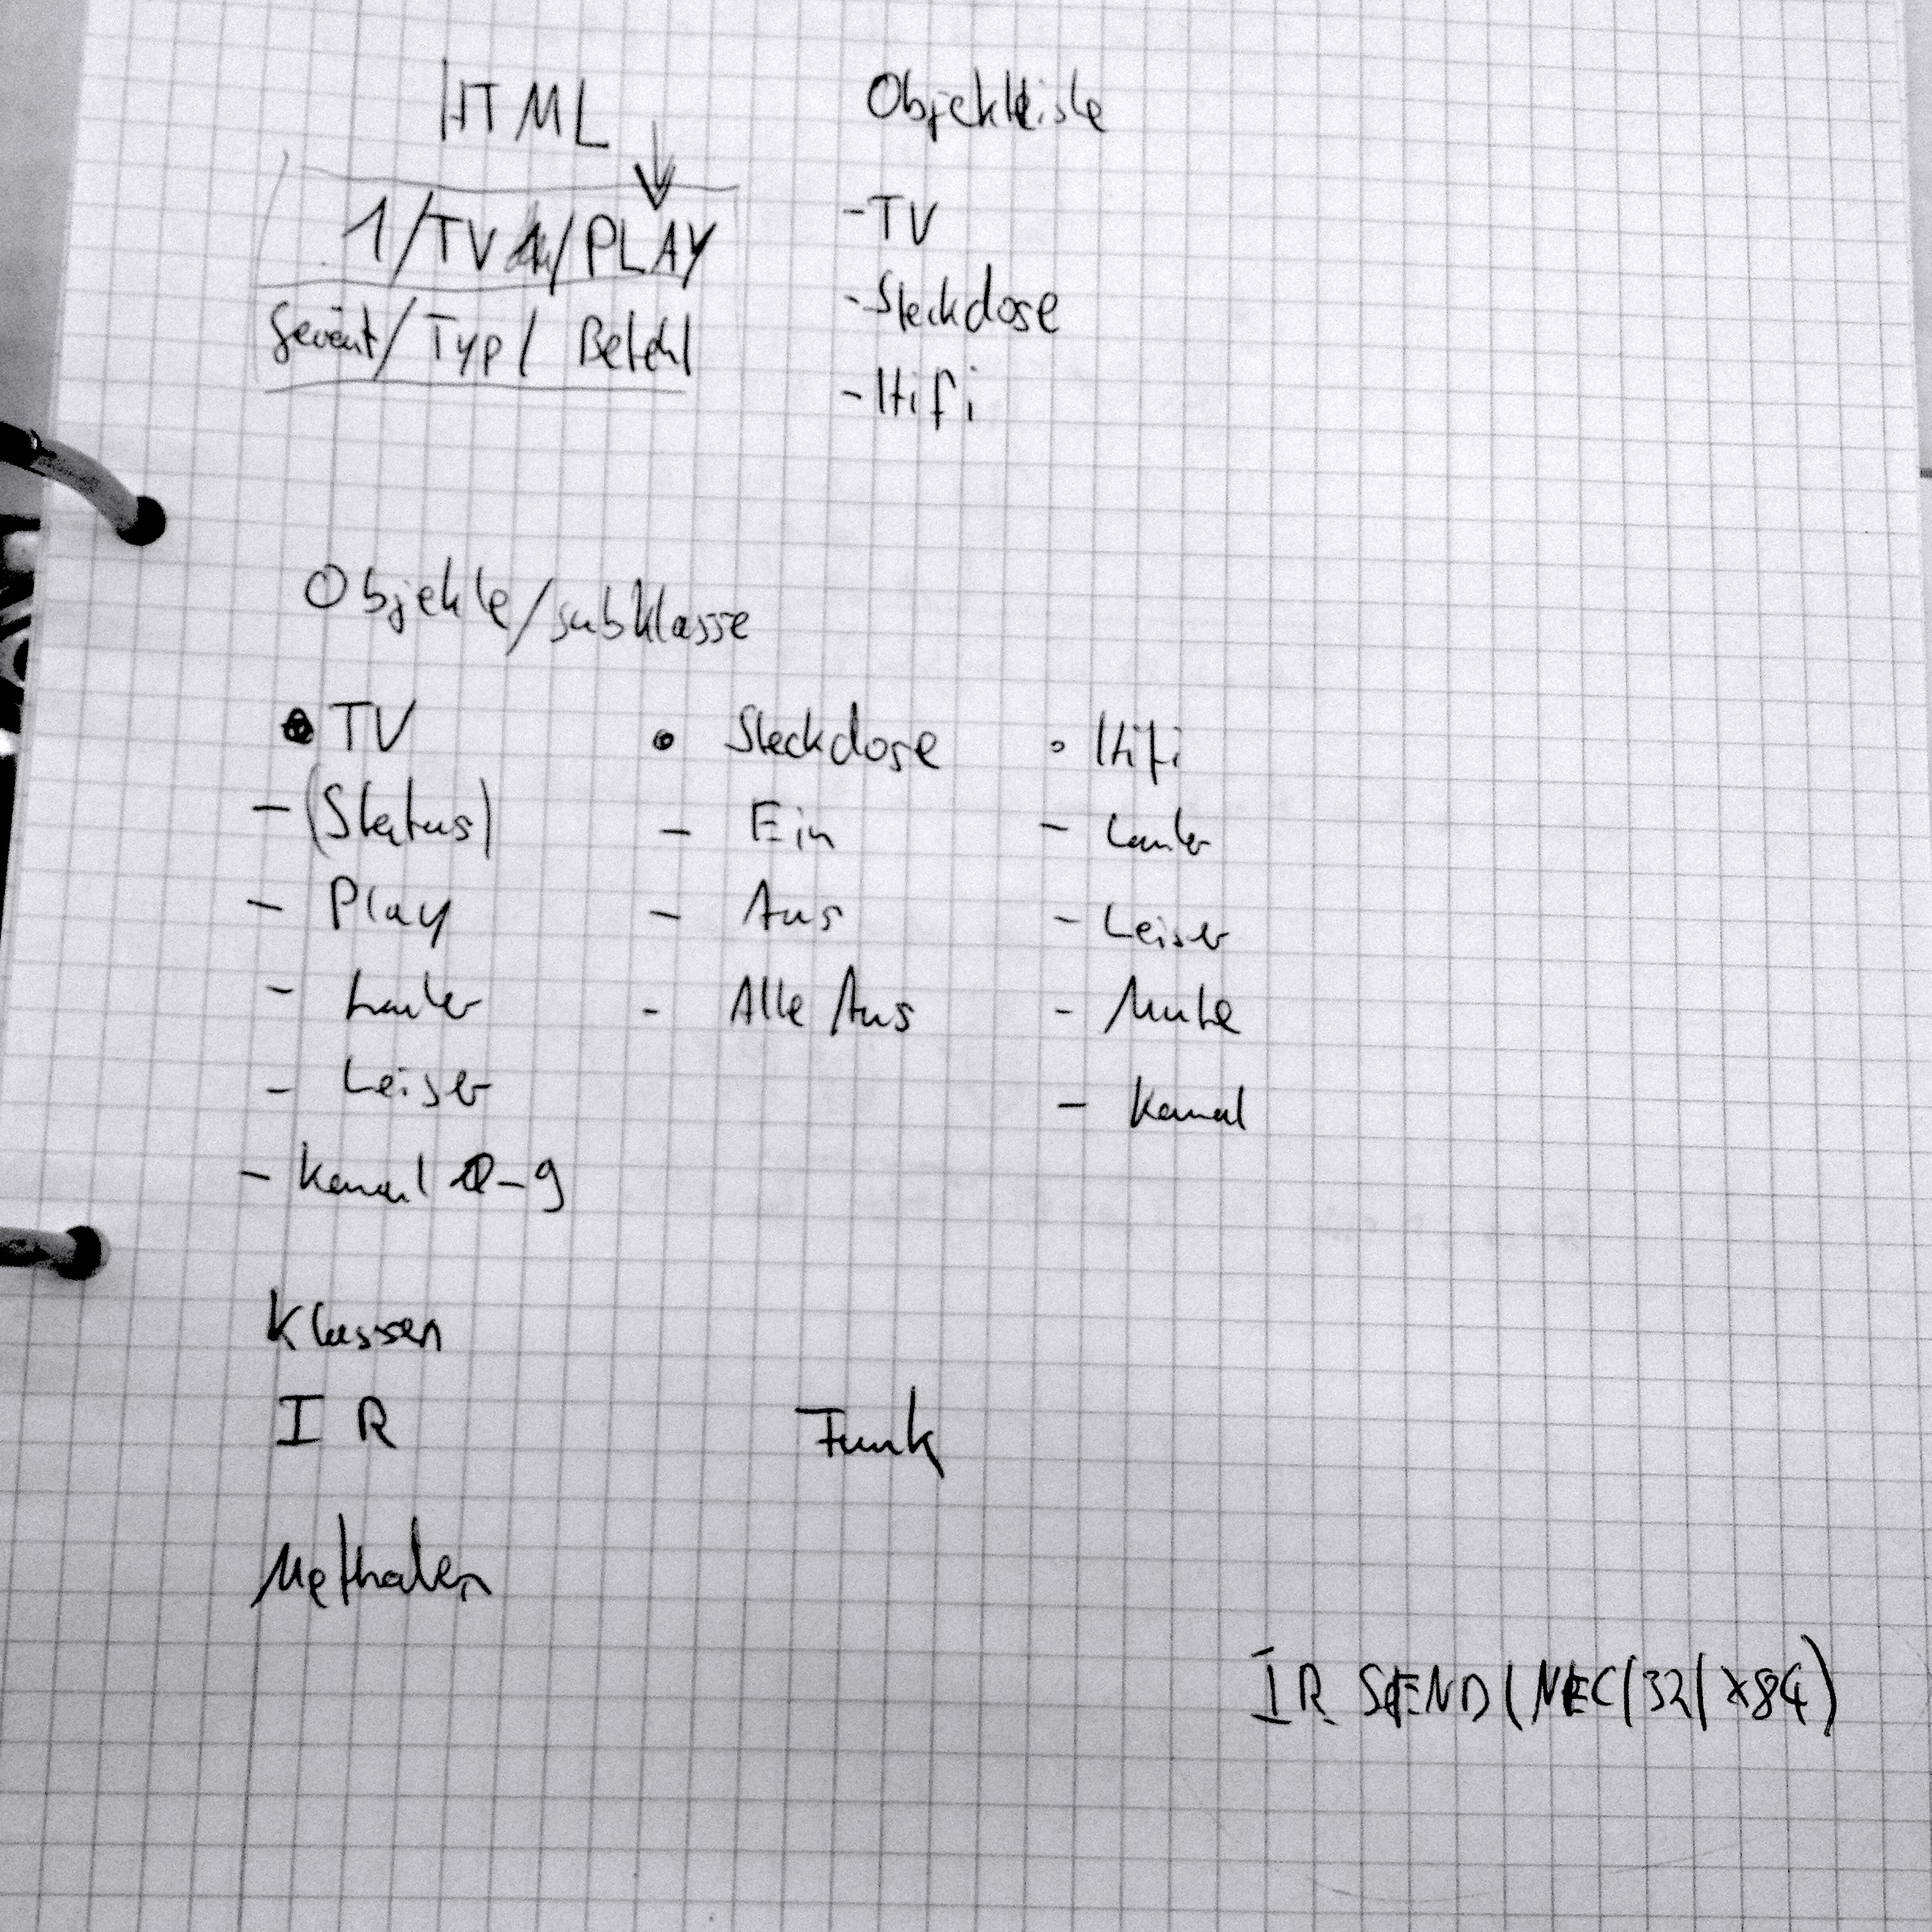
\includegraphics[width=\textwidth]{images/Stuktur-Sketch.jpg}


% Globals: include all pages, don't auto scale
\includepdfset{pages=-,noautoscale}

% Include the PDF files, scaling as required
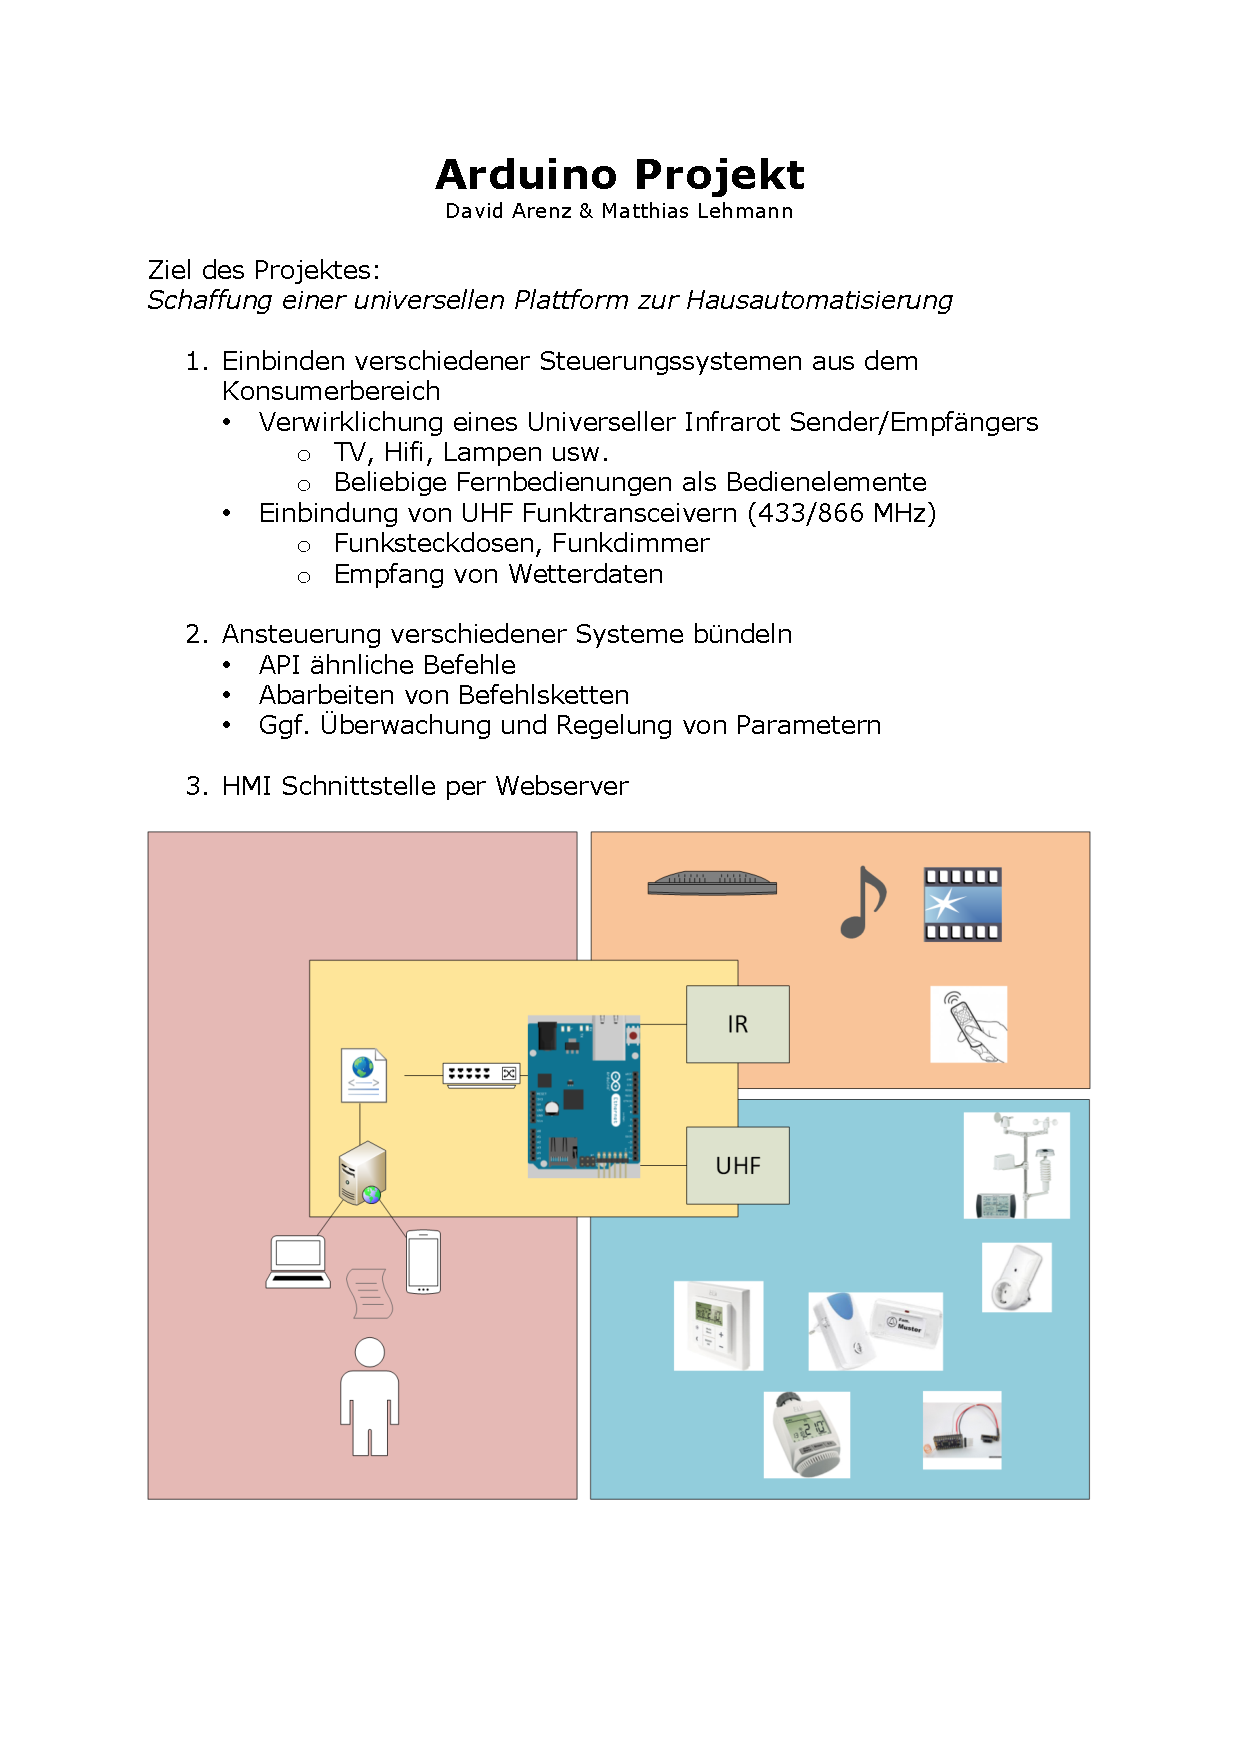
\includepdf{Arduino-Projekt-Overview.pdf}

\section{SD Karte}

Problem: Fehler: Initialisierung der SD-Karte fehlgeschlagen!

Loesung: SD Karte komplett entfernen, SD Karte einstecken, 3s lang den REST Button druecken


\section{Code}
\subsection{WEB\_SD\_IR.ino}
	\mylisting[language=C]{../code/WEB_SD_IR/WEB_SD_IR.ino}
\newpage
\section{Beispiele}
\subsection{InfraredDumper.ino}
	\mylisting[language=C]{../example/InfraredDumper/InfraredDumper.ino}
\newpage
\subsection{InfraredProxy.ino}
	\mylisting[language=C]{../example/InfraredProxy/InfraredProxy.ino}
%\subsection{SDWebServer.ino}
%	\mylisting[language=C]{../example/SDWebServer/SDWebServer.ino}
	

\end{document}